%!TEX root = thesis.tex
\subsection{Dichte} % (fold)
\label{sub:dichte}
Die hier behandelten Graphen haben 100 000 Knoten bei einem minimalen Knotengrad von 1. Nach oben ist der Knotengrad nicht beschränkt. Als Dichte wird hier das Verhältnis von Kanten zu Knoten bezeichnet. Dieses Verhältnis ist gleichzeitig der durschnittliche Knotengrad. Der Knotengrad ist auf nur 100 000 beschränkt, um sehr dichte Graphen trotzdem noch in den Hauptspeicher zu bekommen. Die vollständigen Ergebnisse der Testreihe sind unter \ref{Anhang-Messwerte-Dichte} anggehängt.

Die Messergebnisse liefern kein eindeutiges Bild. Aus Abbildung \ref{fig:max_speedup} ist leicht ersichtlich, dass eine mindeste Graphgröße vorhanden sein muss, damit es sich überhaupt lohnt, parallel an einer Instanz des BFS zu arbeiten. Dabei scheint nicht nur die Anzahl der Knoten relevant zu sein, sondern auch die Anzahl der Kanten. Auffällig ist, dass der Speedup mit steigender Dichte nicht wächst. Der maximal erreichte Speedup liegt bleibt im Bereich zwischen 1.2 und 1.3, bis auf den einen Aussetzer. Der Aussetzer ist ohne weiter Analyse des Graphen nicht zu erklären. Es ist unwahrscheinlich, dass gerade bei einer bestimmten Graphdichte die Parallelisierung dermaßen viel besser funktioniert, als bei allen anderen Graphdichten. Wahrscheinlicher ist es, dass der Zufallsgenerator einen Graph generiert hat, der wenig Kanten zwischen Knoten hat, die auf unterschiedlichen Places liegen. Es kann auch sein, dass durch Zufall die Last auf den Places bei diesem Graph eher gleichmäßig verteilt ist. 

In Abbildung \ref{fig:verteilung_dichte} ist der Speedup von 4 beispielhaft gewählten Graphen aus der Testreihe über dem Grad der Parallelität aufgetragen. Es ist deutlich zu sehen, wie schlecht der 1D-Algorithmus mit dem durchschnittlichen Knotengrad von 5 performt. Auch ist zu sehen, wie ähnlich die Speedup bei 500 und 2000 verläuft, dass also scheinbar ab einer bestimmten Grenze, die bei den Tests bei ca. 500 lag, kein verbesserter Speedup mehr allein durch dichtere Graphen erreichbar ist. Im Kapitel \ref{sub:verteilung} ist nachzulesen, dass die hier gewählten Grenzen des Knotengrads nicht ideal für die Parallelsierung sind. Ob der durchschnittliche Knotengrad einen stärkeren Einfluss hat, wenn der Graph gleichmäßiger ist, müssen weitere Tests zeigen.

\begin{figure}
	\centering
	\label{fig:max_speedup}
	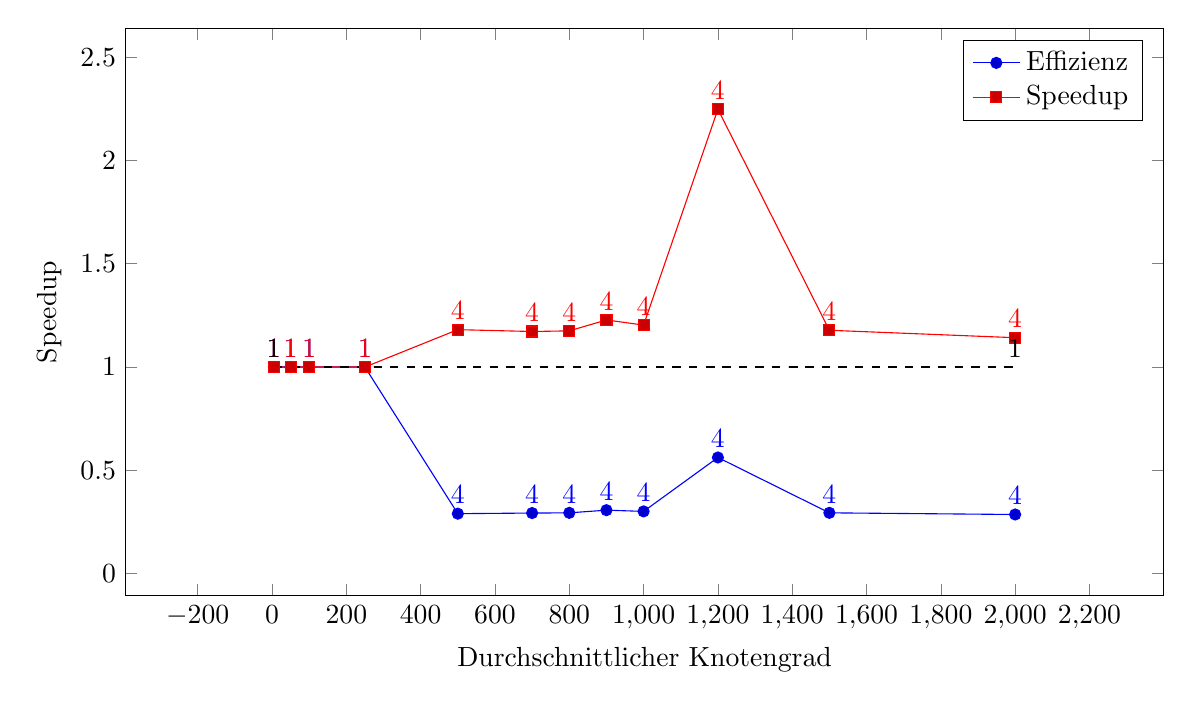
\begin{tikzpicture}
		\begin{axis}[nodes near coords,
			enlargelimits=0.2,
			width=420, height=250,
			xlabel=Durchschnittlicher Knotengrad,
	        ylabel=Speedup]

		    \addplot+[	        
		        point meta=explicit symbolic]
		    coordinates {
		        (5,1) [1]
		        (50,1) [1]
		        (100,1) [1]
		        (250,1) [1]
		        (500,0.29) [4]
		        (700,0.293) [4]
		        (800,0.294) [4]
		        (900,0.307) [4]
		        (1000,0.301) [4]
		        (1200,0.562) [4]
		        (1500,0.294) [4]
		        (2000,0.286) [4]
		    };
		    \addlegendentry{Effizienz}

		    \addplot+[
		        point meta=explicit symbolic]
		    coordinates {
		        (5,1) [1]
		        (50,1) [1]
		        (100,1) [1]
		        (250,1) [1]
		        (500,1.181) [4]
		        (700,1.172) [4]
		        (800,1.175) [4]
		        (900,1.228) [4]
			    (1000,1.203) [4]
			    (1200,2.248) [4]
			    (1500,1.178) [4]
			    (2000,1.142) [4]
			};
		    \addlegendentry{Speedup}

		    \addplot+[
		        smooth,
		        dashed,
		        black,
		        mark=none]
		    coordinates {
		    	(5,1)
		    	(2000,1)
		    };

		\end{axis}
	\end{tikzpicture}
\end{figure}

\begin{figure}
	\centering
	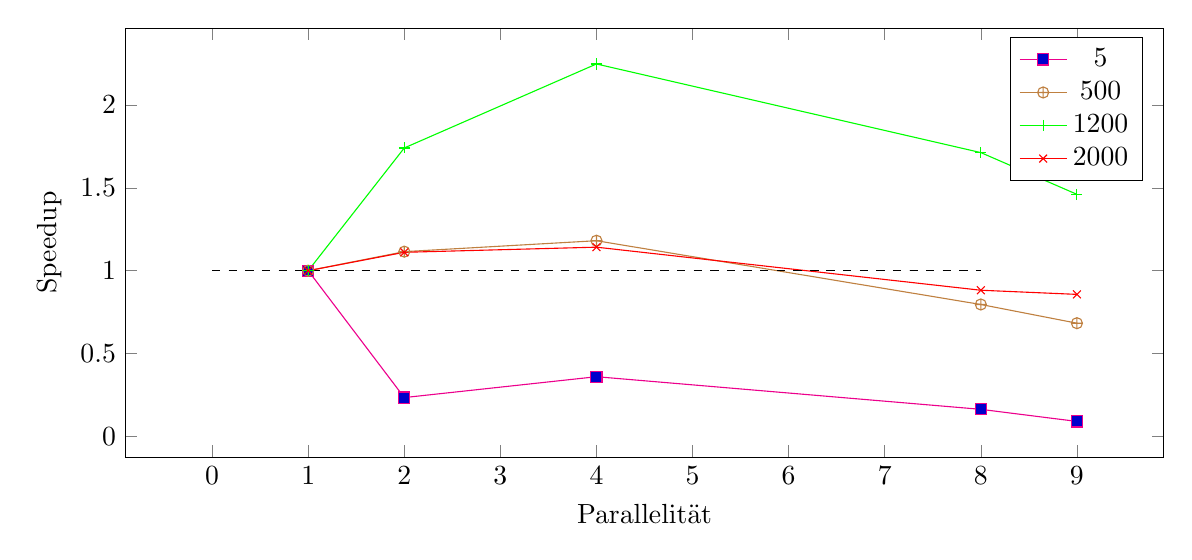
\begin{tikzpicture}
		\begin{axis}[
	        xlabel=Parallelität,
	        ylabel=Speedup,
	        width=420, height=200]

		    \addplot+[
		    magenta,
		    solid,
		    mark=square*]
		    coordinates {
		        (1,1)
		        (2,0.234)
		        (4,0.36)
		        (8,0.163)
		        (9,0.090)
		    };
		    \addlegendentry{5}

		    \addplot+[
		    brown,
		    solid,
		    mark=oplus]
		    coordinates {
		        (1,1)
		        (2,1.115)
		        (4,1.181)
		        (8,0.796)
		        (9,0.683)
		    };
		    \addlegendentry{500}

		    \addplot+[
		    green,
		    solid,
		    mark=+]
		    coordinates {
		        (1,1)
		        (2,1.741)
		        (4,2.248)
		        (8,1.713)
		        (9,1.461)
		    };
		    \addlegendentry{1200}

		    \addplot+[
		    red,
		    solid,
		    mark=x]
		    coordinates {
		        (1,1)
		        (2,1.111)
		        (4,1.142)
		        (8,0.882)
		        (9,0.857)
		    };
		    \addlegendentry{2000}

		    \addplot+[
		        smooth,
		        dashed,
		        black,
		        mark=none]
		    coordinates {
		    	(0,1)
		    	(8,1)
		    };

		\end{axis}
	\end{tikzpicture}
	\caption{Speedup des 1D-Algorithmus über Anzahl der Places. Die Dichte variiert. Als Referenzwert wurde jeweils der schnellste serielle Algorithmus genommen. Es wurden immer die schnellsten, gemessenen Werte verwendet.}
	\label{fig:verteilung_dichte}
\end{figure}
% subsection dichte (end)